% Draft manuscript. Build: latexmk -pdf cnavier_schemes.tex (from docs/paper)
%
% Before submission:
%  - the structured literature search is complete (literature_review.md)
%  - references were checked against Crossref, arXiv or publisher metadata;
%    San & Staples 2012 was checked against the full text (arXiv:1212.0920)
%  - full texts still to be read before submission: Park, Yoo & Choi 2004
%    (currently cited from the abstract); Lee & Seo 2002, JCP 183, 438
%    (not cited because the text was not available); Kawai et al. 2026,
%    Sinhababu & Ayyalasomayajula 2021, Raeth & Hallatschek 2024,
%    Herring et al. 1974, Browning & Kreiss 1989 and Vreman et al. 1996
%  - Zang 1991 and Blaisdell et al. 1996 are used for the skew-symmetric
%    formulation; their abstracts were withheld by the publisher
%  - affiliation, funding, data/code DOI and journal formatting are pending
%  - add the declaration on AI-tool use required by the target journal
\documentclass[11pt,a4paper]{article}
\usepackage[margin=2.5cm]{geometry}
\usepackage[T1]{fontenc}
\usepackage[utf8]{inputenc}
\usepackage{lmodern}
\usepackage{microtype}
\usepackage{amsmath,amssymb}
\usepackage{booktabs}
\usepackage{graphicx}
\usepackage{hyperref}
\usepackage{cleveref}
\graphicspath{{../figures/}}
\newcommand{\Rey}{\mathrm{Re}}
\newcommand{\code}[1]{\texttt{#1}}
\title{Compact and pseudospectral differentiation in two-dimensional turbulence\
\large Dissipation-scale resolution, cell Reynolds number and a dealiased control}
\author{Leonardo Araujo}
\date{Draft, \today}
\begin{document}
\maketitle
\begin{abstract}
San and Staples (2012) compared high-order finite-difference schemes with a Fourier--Galerkin method for decaying two-dimensional turbulence, using the cell Reynolds number $\Rey_c$ to characterize resolution. In the present work this comparison is revisited using explicit sixth-order differences, Lele's compact sixth-order scheme and pseudospectral differentiation. The spectral formulation is considered without dealiasing, with the 2/3 rule and with $3/2$ padding. All methods share the same solver and are represented by their Fourier symbols. Sparse and Fourier implementations of the explicit scheme agree to round-off, while the cost comparison uses the fastest implementation available for each method. Accuracy is measured by the spectral bandwidth that remains within a prescribed tolerance of $2048^2$ explicit sixth-order reference calculations. The most demanding references are also computed with the compact scheme. Cost at equal resolved bandwidth is estimated from GPU step times, the advective stability limit and the measured variation of resolved bandwidth with grid size.
Five decaying cases are computed on two grids. Cases having the same $\Rey_c$ can belong to different resolution regimes. A better organization is obtained with the realized enstrophy-dissipation scale, expressed by $k_{\max}l_\eta$ and evaluated a posteriori from the reference. For $k_{\max}l_\eta\lesssim1$, the grid is under-resolved for every method according to this criterion; explicit sixth order gives the smallest spectral-bandwidth error and the lowest cost. Compact sixth order performs best for approximately $1\lesssim k_{\max}l_\eta\lesssim2$, resolving $1.3$--$1.6$ times the bandwidth of explicit sixth order where $k_{\max}l_\eta\gtrsim1$, with an estimated equal-range cost of $0.44$--$0.81$ times that of the explicit scheme. Once $k_{\max}l_\eta$ reaches about $2$--$2.5$, pseudospectral differentiation becomes the leading method and resolves as much as $1.7$ times the explicit bandwidth at $0.54$--$0.76$ times its cost.
The changes of leading scheme occur near the usual thresholds for resolved ($k_{\max}l_\eta>1$) and well-resolved ($k_{\max}l_\eta\ge2$) two-dimensional simulations, although these limits are inferred from the same ten points used to obtain the ordering. Pseudospectral calculations also exhibit an accumulation of energy near the cutoff. Removing quadratic aliasing with $3/2$ padding changes the resolved bandwidth by at most eight shells in the ten cases and does not remove the pile-up, while increasing the step cost by a factor of $1.85$. Thus, for the skew-symmetric nonlinear form considered here, the compact--spectral crossover cannot be attributed to quadratic aliasing of the nonlinear term. The organization found for transient decaying turbulence does not extend directly to all flow statistics. In a statistically stationary forced case with $k_{\max}l_\eta=1.33$, the methods cannot be distinguished in the inertial range within the sampling scatter of the forcing.
\end{abstract}
% =============================================================================
\section{Introduction}
% =============================================================================
High-order finite-difference schemes are commonly used in numerical simulations of turbulent flows because they can retain good small-scale resolution while remaining local in physical space. Compact finite differences are a notable example. In the schemes introduced by Lele~\cite{lele1992}, derivatives are obtained from an implicit tridiagonal relation whose modified wavenumber remains close to the exact value through a large portion of the represented spectrum. This behavior is usually referred to as spectral-like resolution.
Laizet and Lamballais~\cite{laizet2009} applied this approach to incompressible-flow simulations using sixth-order compact differences, modified-wavenumber representations of the numerical operators and a Poisson equation treated in spectral space. Their tests showed that compact schemes retain small-scale quantities considerably better than second-order methods at marginal resolution, while requiring only a moderate additional cost. They also reported compact differentiation of the nonlinear terms to be less expensive than a pseudospectral treatment. This numerical approach later formed the basis of Incompact3d~\cite{laizet2011,laizet2010}, which was developed for simulations on up to $O(10^5)$ computational cores, and of the open-source Xcompact3d framework~\cite{bartholomew2020}. The use of compact finite differences as a quasi-spectral alternative is consequently well established.
Comparisons between finite-difference and spectral methods in two-dimensional turbulence precede these developments. Fox and Orszag~\cite{fox1973} used a pseudospectral approximation for two-dimensional turbulence, while Herring et al.~\cite{herring1974} reported that a spectral calculation could provide an accuracy comparable to that of a grid-point method having twice the resolution. Browning and Kreiss~\cite{browning1989} constructed converged pseudospectral reference solutions from an estimate of the smallest relevant scale. When the energy remained concentrated at low wavenumbers, their fourth-order solution on the same grid was nearly indistinguishable from the reference, whereas truncated and hyperviscous calculations showed larger differences.
Numerical errors become more important as the flow approaches the grid cutoff. Ghosal~\cite{ghosal1996} and Kravchenko and Moin~\cite{kravchenko1997} examined truncation and aliasing errors in large-eddy simulations and showed that aliasing can be particularly harmful for spectral and high-order finite-difference methods. The formulation of the nonlinear term also affects conservation in the presence of these errors. Moin and Mahesh~\cite{moin1998} summarized the balance in simple terms: finite differences generally introduce larger differentiation errors, but lower aliasing errors. Scheme ranking is therefore not fixed. Vreman et al.~\cite{vreman1996}, for example, found a reversal between second- and fourth-order methods when the ratio between the filter width and the grid spacing was changed. Fedioun et al.~\cite{fedioun2001} separated truncation from aliasing effects and obtained compact finite-difference results close to a dealiased pseudospectral solution for decaying isotropic turbulence. Park et al.~\cite{park2004} likewise found the finite-differencing error to be larger than the aliasing error in their large-eddy simulations, with both errors reduced by a skew-symmetric nonlinear formulation.
A particularly close comparison was performed by San and Staples~\cite{san2012}. Their calculations used the vorticity--streamfunction form of the two-dimensional equations and a common fast Poisson solver. Explicit central differences from second to sixth order, fourth- and sixth-order compact differences, Arakawa and dispersion-relation-preserving schemes were compared with a Fourier--Galerkin method. The sixth-order methods agreed closely with the spectral calculation while giving CPU speed-ups of approximately five. Resolution was classified using the cell Reynolds number, $\Rey_c=\Rey h$ ($\Rey 2\pi/N$ in their domain). All methods agreed below approximately $\Rey_c=2$. Differences increased with $\Rey_c$, and above about $30$ the non-conservative methods developed a small-scale energy pile-up. This behavior was attributed to aliasing and was absent with the conservative Arakawa scheme. Their spectral calculation was dealiased by padding to $2N$, while its computational cost was obtained by interpolation between timings at $N$ and $2N$ points.
Later work provides other ways of looking at the same problem. Direct simulations are normally judged by the relation between the numerical cutoff and the dissipative scale. The familiar three-dimensional quantity is $k_{\max}\eta$~\cite{yeung2018}. In two dimensions, Lunasin et al.~\cite{lunasin2007} used the enstrophy-dissipation length $l_\eta=(\nu^3/\eta)^{1/6}$ and classified simulations with $k_{\max}l_\eta>1$ as resolved and those with $k_{\max}l_\eta\ge2$ as well resolved. Spectral decay at the cutoff has also been used as a convergence test. Baty~\cite{baty2026}, for instance, uses a cutoff-to-peak spectral ratio in two-dimensional pseudospectral magnetohydrodynamics. Kritsuk et al.~\cite{kritsuk2011} compared numerical schemes through an effective spectral bandwidth defined by agreement with a high-resolution reference. In the structured search performed for the present study, no previous use of these quantities was found as a criterion for selecting among differentiation schemes.
The interpretation of high-wavenumber pile-up is less direct. Aliasing is a usual explanation~\cite{fontana2020}, but accumulation near a spectral cutoff is not restricted to aliased calculations. Galerkin-truncated systems can thermalize at high wavenumbers~\cite{cichowlas2005,frisch2008,ray2011}, and Bardos and Tadmor~\cite{bardos2015} showed that the 2/3-dealiased Fourier method can lose spectral convergence once the solution ceases to be smooth. Ishihara et al.~\cite{ishihara2018} described high-wavenumber accumulation in alias-free spectral calculations as a truncation effect not present in their finite-difference results, while Yalla et al.~\cite{yalla2021} related a similar pile-up in implicitly filtered large-eddy simulation to numerical dispersion. No controlled comparison was found in which the same marginally resolved flow was computed both with and without $3/2$ padding in order to separate these effects directly.
Computational efficiency adds another part to the comparison. Spectral and finite-difference methods have long been compared in terms of cost and accuracy~\cite{fornberg1987}. More recently, effective spectral resolution has been combined with computational resources and a stability-limited time step~\cite{kawai2026}. The stable time step itself depends on the discretization and on the form chosen for the nonlinear term~\cite{raeth2024}. Dealiasing methods also have different costs for a given accuracy~\cite{sinhababu2021,lambert2026}. In forced three-dimensional turbulence, Rodhiya et al.~\cite{rodhiya2026} obtained nearly the same statistics with pseudospectral and second-order finite-difference solvers. For channel flow, Yamamoto and Tsuji~\cite{yamamoto2026} found that selective filtering gave a better cost--accuracy balance than full $3/2$ dealiasing.
The present study addresses three related questions. First, does the cell Reynolds number provide the most useful parameter for comparing differentiation schemes, or is the realized dissipation scale of the flow more relevant? Second, does the spectral pile-up observed near the resolution limit remain after quadratic aliasing is removed? Finally, how do the schemes compare when computational cost includes both the work per step and the time-step restriction?
To answer these questions, all discretizations are incorporated in one solver. Pseudospectral differentiation is treated as one of the methods being tested rather than as the reference, and is evaluated without dealiasing, with the 2/3 rule and with $3/2$ padding. High-resolution reference calculations are checked with a second differentiation scheme. The cost comparison uses the fastest implementation of each method and includes its advective stability limit.
No new differentiation scheme is proposed here. The purpose is to compare existing methods under the same numerical framework and determine how their relative performance changes with resolution. The comparison uses a reference-based spectral bandwidth, examines its dependence on $\Rey_c$ and $k_{\max}l_\eta$, tests the pseudospectral result with explicit dealiasing, and repeats the analysis for forced statistically stationary turbulence.
% =============================================================================
\section{Numerical method}
\label{sec:method}
% =============================================================================
\subsection{Equations and time integration}
The two-dimensional incompressible Navier--Stokes equations are solved in a doubly periodic unit square using the vorticity--streamfunction formulation,
\begin{equation}
\frac{\partial\omega}{\partial t}=N(\omega)+\nu\nabla^2\omega+f,\qquad
\nabla^2\psi=-\omega,\qquad u=\partial_y\psi,\quad v=-\partial_x\psi,
\end{equation}
where $\nu=1/\Rey$. The term $f$ contains the forcing and damping contributions described in \cref{sec:forced}. The nonlinear term is written in skew-symmetric form,
\begin{equation}
N=-\tfrac12\left(u,D_x\omega+v,D_y\omega\right)
  -\tfrac12\left(D_x(u\omega)+D_y(v\omega)\right).
\label{eq:skew}
\end{equation}
For periodic antisymmetric difference operators, this form conserves the discrete enstrophy $\tfrac12\langle\omega^2\rangle$ to round-off for all schemes considered. The purely advective form does not. In the under-resolved tests reported in the companion methodology, it produces spurious enstrophy near the cutoff corresponding to $23$--$45,%$ of the input. Time integration is performed with the classical fourth-order Runge--Kutta method, using double precision.
\subsection{Operators in Fourier space}
For a periodic grid with $n$ points, any translation-invariant difference operator forms a circulant matrix and is diagonal in the discrete Fourier basis. For a stencil with coefficients $c_j$, the corresponding eigenvalue at wavenumber $k$ is
$\sum_jc_je^{ikjh}$. The first- and second-derivative symbols are written as
$\tilde D_x(k)=ik^*(k)$ and $\tilde D_{xx}(k)=-(k^{**})^2$, respectively. Thus each discretization can be represented by its set of modified wavenumbers.
The one-dimensional operator symbols are stored in a common table. This same table is used throughout the solver to construct the Poisson eigenvalues $\tilde D_{xx}+\tilde D_{yy}$, the modal energy used in the diagnostics, the amplitudes of the random forcing and the stability limits. Consequently, changing the differentiation method changes the symbols, while the remaining numerical machinery is unchanged.
The Fourier implementation starts with one transform of $\omega$. Inverse transforms of the corresponding products provide $D_x\omega$, $D_y\omega$, the Laplacian, the stream function and the velocity components. Two additional forward transforms and one inverse transform are required by the skew-symmetric correction. For a finite-difference method, this procedure applies exactly the same circulant matrix as the corresponding sparse stencil. The two implementations were compared after 20 steps of a forced calculation with all terms enabled and agreed to $10^{-14}$. The time integrator, forcing, diagnostics, nonlinear formulation and scheme-consistent Poisson operator are common to all cases.
\subsection{Differentiation schemes}
\begin{description}
  \item[Explicit sixth order (E6).] The first and second derivatives are represented by the centered seven-point sixth-order stencils.
  \item[Compact sixth order (C6).] Lele's tridiagonal compact schemes~\cite{lele1992} are used. For the first derivative,
  $\tfrac13f'_{i-1}+f'i+\tfrac13f'{i+1}
  =\tfrac{14}{9}\delta_1f_i+\tfrac19\delta_2f_i$,
  with the analogous second-derivative formulation using $\alpha=2/11$.
  On a periodic grid $A^{-1}B$ is circulant. Its symbols are
  $k^*h=(\tfrac{14}9\sin\theta+\tfrac1{18}\sin2\theta)/(1+\tfrac23\cos\theta)$
  and
  $(k^{**}h)^2=-(\tfrac{24}{11}(\cos\theta-1)+\tfrac3{22}(\cos2\theta-1))/(1+\tfrac4{11}\cos\theta)$,
  with $\theta=kh$.
  \item[Pseudospectral (S).] Exact differentiation is obtained with the symbols $ik$ and $-k^2$. The first-derivative symbol is set to zero at the Nyquist wavenumber. For these symbols, the discrete kinetic energies $\tfrac12\langle|\mathbf u|^2\rangle$ and $\tfrac12\langle\psi\omega\rangle$ are identical.
  \item[Pseudospectral with the 2/3 rule (S$_{2/3}$).] Orszag's truncation~\cite{orszag1971} is applied by removing modes satisfying $|k|\ge n/3$ in either coordinate direction from the operators and from $\omega$ after each step. The resulting nonlinear term is a Galerkin truncation. Energy and enstrophy are conserved to round-off in either nonlinear form, with residual transfers of about $10^{-14}$ relative to the largest shell transfer in the tests.
  \item[Padded pseudospectral (S$_{3/2}$).] The exact spectral symbols are retained, while the nonlinear product is dealiased using $3/2$ padding~\cite{canuto2006}. The spectra of $u$, $v$, $D_x\omega$ and $D_y\omega$ are extended with zeros to a grid $3/2$ as fine, the products are formed on that grid, and the resulting spectra are truncated back to the original resolution. Except for the Nyquist modes, the retained modes therefore contain the quadratic Fourier--Galerkin nonlinear term without aliasing. Unlike the 2/3 rule, no retained non-Nyquist mode is discarded.
\end{description}
\begin{figure}[t]
\centering
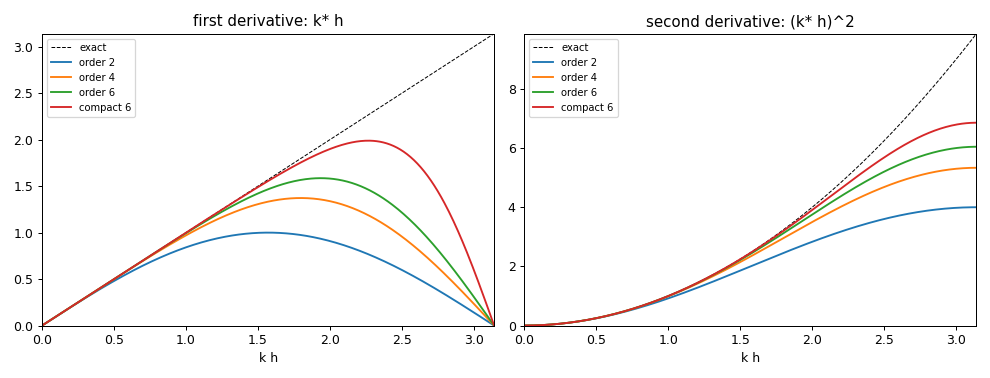
\includegraphics[width=0.85\textwidth]{modified_wavenumber.png}
\caption{Modified wavenumbers for the first and second derivatives. Explicit schemes of orders 2, 4 and 6 and the sixth-order compact scheme are shown. Dashed lines indicate the exact pseudospectral symbols.}
\label{fig:kstar}
\end{figure}
\begin{table}[t]
\centering\small
\begin{tabular}{lccccc}
\toprule
& \multicolumn{2}{c}{first derivative} & \multicolumn{2}{c}{second derivative} & \
fraction of $0,\pi$ within & $1,%$ & $10,%$ & $1,%$ & $10,%$ & $(k^*h){\max}$ \
\midrule
E6 & 0.35 & 0.54 & 0.45 & 0.71 & 1.59 \
C6 & 0.50 & 0.70 & 0.56 & 0.81 & 1.99 \
S & 1 & 1 & 1 & 1 & $\pi$ \
S${3/2}$ & 1 & 1 & 1 & 1 & $\pi$ \
S$_{2/3}$ & 2/3 & 2/3 & 2/3 & 2/3 & $2\pi/3$ \
\bottomrule
\end{tabular}
\caption{Portion of the represented interval differentiated with errors below $1,%$ and $10,%$, together with the largest modified wavenumber. The last quantity determines the relative advective stability limit.}
\label{tab:kstar}
\end{table}
The modified-wavenumber curves are shown in \cref{fig:kstar}, and the corresponding numerical ranges are summarized in \cref{tab:kstar}. Methods that remain accurate farther into the spectrum also have larger values of $(k^*h){\max}$. Their explicit advective time-step limit is therefore smaller, varying as $h/(k^*h){\max}$.
\subsection{Spectral diagnostics}
All spectral diagnostics use the operators of the active scheme. For a mode $\mathbf k$, the energy is written as $\tfrac12A|\hat\psi|^2$, where
$A=|\tilde D_x|^2+|\tilde D_y|^2$ and
$\hat\omega=Q\hat\psi$, with
$Q=-(\tilde D_{xx}+\tilde D_{yy})$.
The energy and enstrophy fluxes are computed from the same nonlinear term used by the solver. The energy transfer is weighted by $A/Q$. With this definition, the discrete energy balance closes to round-off rather than only to the formal order of the scheme. Spectra $E(k)$ are obtained by summing the modal energies in shells of width $2\pi$.
% =============================================================================
\section{Verification}
\label{sec:verification}
% =============================================================================
The spatial orders were first checked with a manufactured periodic solution. The explicit schemes recover orders 2, 4 and 6, while C6 gives an observed order of $6.04$. At $64^2$, the C6 error is twelve times smaller than the E6 error. For the pseudospectral case, the error at $32^2$ is $3.5\times10^{-9}$, compared with $1.1\times10^{-4}$ for C6. Halving the time step reduces the pseudospectral error by a factor of 16, showing that the remaining error is controlled by RK4.
The two implementations of the finite-difference operators were also compared. For E6 and C6, applying the operators through Fourier symbols reproduces the sparse formulation to $10^{-14}$ in the fields, integral quantities and spectra after 20 forced steps. In a complete decaying-turbulence calculation, the C6 spectrum obtained in Fourier space agrees with that of the exact banded implementation to $4\times10^{-12}$.
The padded nonlinear term was verified independently against direct convolution of the modal coefficients. On $10\times8$ and $9\times7$ grids, covering even and odd Nyquist cases, agreement over the non-Nyquist triads is $7\times10^{-15}$. The GPU implementation based on cuFFT reproduces the FFTW CPU results to $6\times10^{-15}$ for all five methods. In addition, the skew-symmetric form conserves enstrophy to approximately $10^{-15}$--$10^{-14}$ of the largest shell transfer. The S${2/3}$ and S${3/2}$ formulations also conserve energy to this level in either nonlinear form.
Each decaying case uses its own $2048^2$ E6 reference. To check that the comparison is not controlled by the reference discretization, the two most demanding cases, $\Rey=8\times10^4$ and $k_0=20$, were repeated at $2048^2$ with C6. The two references differ by no more than $1.5\times10^{-3}$ through $K=255$, which is the largest shell used in the comparison, and by approximately $10^{-4}$ through $K=127$. These differences are well below the $2,%$ and $10,%$ error levels used to define the resolved bandwidth.
% =============================================================================
\section{Experimental design}
\label{sec:design}
% =============================================================================
\paragraph{Decaying turbulence.}
The baseline calculation uses $\Rey=2\times10^4$ and $k_0=10$. Reynolds number and initial spectral location are then changed separately, with $\Rey=5\times10^3$ and $8\times10^4$, or $k_0=5$ and $20$. Each of the five cases is computed at $256^2$ and $512^2$ with all differentiation schemes.
The initial condition consists of random Fourier phases and modal amplitudes following the shell envelope
$E(k)\propto(k/k_0)^4e^{-2(k/k_0)^2}$, whose maximum occurs at $K=k_0$, with $K=|\mathbf k|/2\pi$. The total initial energy is normalized to $E=\tfrac12$. A phase is determined only by its wavevector and the common random seed, which gives the same initial field on every grid capable of representing the corresponding mode.
All schemes in a given case use the same time step, $6.25\times10^{-5}$, and are therefore compared at the same physical time. Since the initial energy is fixed, the turnover time varies as $\tau_0\propto1/k_0$. The comparison is made at
$t=0.09\cdot10/k_0$, corresponding to approximately six eddy-turnover times. At this stage the cascade has populated the spectrum, while the largest scales, $K\le20$, remain within $10^{-3}$--$10^{-2}$ of the reference. The solutions have therefore not yet decorrelated. At $t=0.5$, by comparison, differences of tens of percent are already present at $K=10$.
\paragraph{Accuracy and resolution parameters.}
The effective bandwidth is defined by the largest shell $K_{10}$ for which every preceding shell remains within $10,%$ of the reference spectrum. A corresponding $K_2$ is obtained with a $2,%$ tolerance. The maximum value of $E/E_{\mathrm{ref}}$ is used to characterize the high-wavenumber pile-up.
Three resolution measures are considered. The first is the cutoff-to-peak energy ratio
\begin{equation}
\chi=\frac{E_{\mathrm{ref}}(K_{\mathrm{Nyq}})}
{\max_K E_{\mathrm{ref}}(K)},
\end{equation}
which measures the amount of spectral energy reaching the Nyquist shell of the coarse grid. Unlike the cell Reynolds number, it depends on the actual distribution of energy in the flow.
For comparison with San and Staples~\cite{san2012}, the cell Reynolds number is defined as $\Rey_c=\Rey h$, with $h=1/n$ for the unit square. Since all present calculations start with the same total energy, $\Rey_c$ can be compared among the present cases, although its numerical value is not the same as in their domain. This quantity contains information about viscosity and grid spacing, but not about $k_0$ or the instantaneous spectrum.
The third parameter is the classical two-dimensional dissipation-scale measure $k_{\max}l_\eta$. Here $k_{\max}=\pi/h$ is the one-dimensional Nyquist wavenumber and
$l_\eta=(\nu^3/\eta)^{1/6}$, where
$\eta=\nu\langle|\nabla\omega|^2\rangle$ is the reference enstrophy-dissipation rate at the comparison time. The shell sum of viscous enstrophy dissipation agrees with $2\nu$ times the palinstrophy to $0.1,%$. This definition of $\eta$ is the same as that used by Lunasin et al.~\cite{lunasin2007}.
Their reported $k_{\max}$ is the largest radial wavenumber retained by the 2/3 rule, $(\sqrt2/3)N$ in units of $2\pi$ for the unit box. If the product $k_{\max}l_\eta$ is formed with angular wavenumbers, as in the usual three-dimensional criterion $k_{\max}\eta$ with $k_{\max}=\pi/\Delta x$, their cutoff is approximately $0.94$ of the present value. The convention is not stated explicitly in their text. Interpreting the tabulated values as shell units instead would imply about 38 grid cells per $l_\eta$ in their resolved calculations, rather than approximately 6 with angular units. The ordering found below is unchanged by this common rescaling; only its numerical correspondence with the published thresholds depends on the convention.
Both $\chi$ and $k_{\max}l_\eta$ are evaluated from the high-resolution reference and should therefore be regarded as a posteriori descriptors in this study. An a priori use of $k_{\max}l_\eta$ for scheme selection would require an estimate of $\eta$ before the reference is known. An under-resolved calculation may not provide such an estimate reliably.
\paragraph{Computational cost.}
Step times $t_{\mathrm{step}}$ are measured in double precision on one NVIDIA RTX 3050 laptop GPU. At the advective stability limit,
$\Delta t\propto h/(k^*h){\max}$.
The cost per unit of physical simulation time is consequently proportional to
$t{\mathrm{step}}(k^*h)_{\max}/h$.
The comparison is made at equal effective bandwidth and is an estimate rather than a direct benchmark of every equivalent-resolution configuration. For the baseline E6 runs, $K_{10}$ increases from 74 shells on $256^2$ to 152 on $512^2$, approximately linearly with $n$. Its cost per unit physical time varies as $n^3$. An E6 calculation matching a method with bandwidth $K_{10}$ therefore has an estimated cost proportional to
$(K_{10}/K_{10}^{\mathrm{E6}})^3$
relative to E6 on the same grid. The reported cost ratio compares each method with this equivalent-bandwidth E6 estimate.
Each method is timed in its fastest implementation available in the solver. C6 and all pseudospectral variants are most efficient in Fourier space. E6 is faster as a sparse seven-point stencil and is therefore computed and timed in that form. Since sparse and Fourier E6 apply the same matrix and agree to $10^{-14}$, this choice changes the cost but not the discretization. It also favors E6; applying it in Fourier space would increase its step cost by about $40,%$.
\paragraph{Forced turbulence.}
Because independently forced simulations decorrelate, their comparison is based on time-averaged statistics rather than instantaneous spectra. Random white-in-time forcing injects energy at a rate $\varepsilon=0.1$ in the shell $|K-4|\le1$, while the inverse cascade is removed by a large-scale hypodrag $-\alpha_h\psi$.
Two $256^2$ cases are considered. In the first, the small-scale dissipation is concentrated near the cutoff using hyperviscosity,
$-\nu_h(-\nabla^2)^4\omega$, and statistics are collected over $t=6$--$16$. The second uses ordinary viscosity at $\Rey=10^5$ without hyperviscosity and is compared with a $768^2$ pseudospectral reference over $t=4$--$10$.
% =============================================================================
\section{Results}
% =============================================================================
\subsection{Decaying turbulence: scheme ordering}
\label{sec:decaying}
\begin{table}[t]
\centering\small
\setlength{\tabcolsep}{4pt}
\begin{tabular}{lcccccccccc}
\toprule
case & grid & $\Rey_c$ & $\chi$ & $k_{\max}l_\eta$ & E6 & C6 & S & S${3/2}$ & S${2/3}$ \
\midrule
$\Rey=8\times10^4$ & $256^2$ & 313 & $1.2\times10^{-5}$ & 0.76 & \textbf{80} & 79 & 75 & 79 & 46 \
$k_0=20$ & $256^2$ & 78 & $1.6\times10^{-4}$ & 0.92 & \textbf{89} & 74 & 74 & 72 & 49 \
baseline & $256^2$ & 78 & $4.9\times10^{-6}$ & 1.35 & 74 & \textbf{118} & 93 & 93 & 50 \
$\Rey=8\times10^4$ & $512^2$ & 156 & $2.3\times10^{-7}$ & 1.52 & 152 & \textbf{217} & 193 & 200 & 117 \
$k_0=20$ & $512^2$ & 39 & $1.6\times10^{-6}$ & 1.83 & 159 & 213 & \textbf{217} & \textbf{217} & 130 \
$k_0=5$ & $256^2$ & 78 & $9.0\times10^{-8}$ & 2.01 & 71 & 105 & 101 & \textbf{109} & 62 \
$\Rey=5\times10^3$ & $256^2$ & 20 & $2.0\times10^{-7}$ & 2.50 & 74 & 105 & \textbf{120} & \textbf{120} & 70 \
baseline & $512^2$ & 39 & $1.5\times10^{-8}$ & 2.71 & 152 & 198 & 235 & \textbf{239} & 143 \
$k_0=5$ & $512^2$ & 39 & $4.2\times10^{-11}$ & 4.01 & 146 & 197 & \textbf{246} & \textbf{246} & 154 \
$\Rey=5\times10^3$ & $512^2$ & 9.8 & $2.8\times10^{-12}$ & 5.01 & 144 & 196 & \textbf{249} & 248 & 163 \
\bottomrule
\end{tabular}
\caption{Resolved spectral bandwidth $K_{10}$ for the decaying cases. The rows are arranged by $k_{\max}l_\eta$. Values of $\Rey_c=\Rey h$ and $\chi$ are included for comparison. The Nyquist shells are 127 for $256^2$ and 255 for $512^2$.}
\label{tab:map}
\end{table}
\begin{figure}[t]
\centering
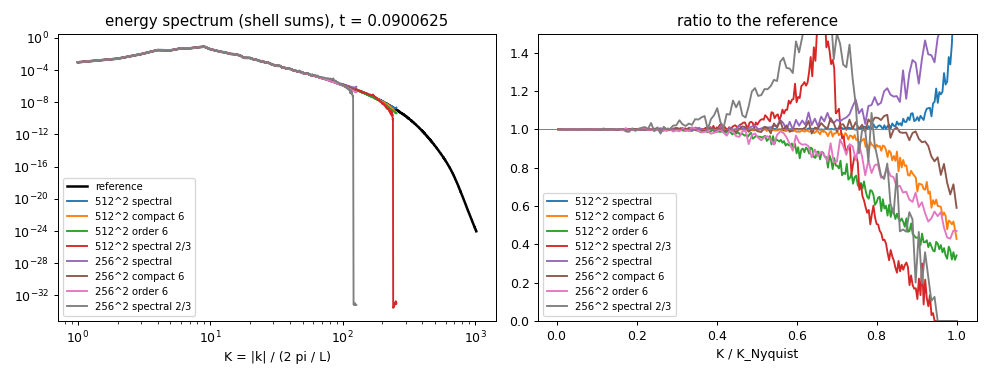
\includegraphics[width=0.95\textwidth]{resolution_fourier.png}
\caption{Energy spectra for the baseline case ($\Rey=2\times10^4$, $k_0=10$) at $t=0.09$, computed on $256^2$ and $512^2$ grids, with ratios to the $2048^2$ reference. The finite-difference spectra decrease below the reference near the cutoff. The undealiased pseudospectral solution instead develops a high-wavenumber excess, reaching approximately twice the reference value at the $256^2$ Nyquist shell. The 2/3 calculation truncates the spectrum earlier and develops a pile-up immediately below its own cutoff.}
\label{fig:baseline}
\end{figure}
\begin{figure}[t]
\centering
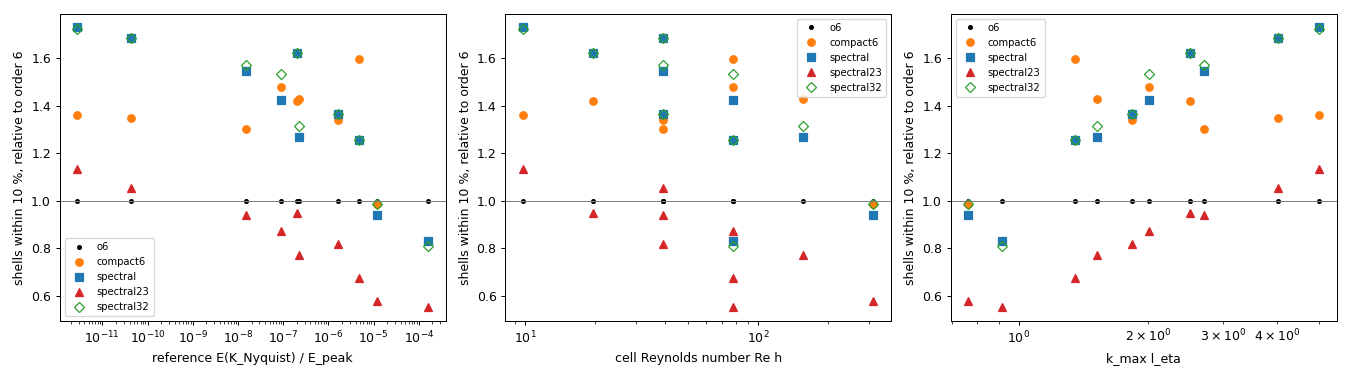
\includegraphics[width=\textwidth]{crossover_rec.png}
\caption{Resolved bandwidth relative to E6 for the five decaying cases on two grids. Results are plotted against the cutoff ratio $\chi$ (left), the cell Reynolds number $\Rey_c=\Rey h$ (middle) and the dissipation-scale resolution $k_{\max}l_\eta$ (right). Open diamonds denote S${3/2}$. Cases at $\Rey_c=39$ and 78 occupy different regimes, whereas the leading scheme varies monotonically when the same data are ordered by $k{\max}l_\eta$.}
\label{fig:map}
\end{figure}
The comparison in \cref{tab:map,fig:map} shows that $\Rey_c$ alone does not organize the results. This can be seen directly from the three $256^2$ calculations having $\Rey_c=78$. Only $k_0$ is changed among them, yet E6 gives the largest bandwidth for $k_0=20$, C6 for $k_0=10$, and C6 and padded pseudospectral differentiation are the leading methods for $k_0=5$. The same behavior appears at $\Rey_c=39$: the pseudospectral bandwidth relative to E6 is $1.68$ for $k_0=5$ and $1.36$ for $k_0=20$.
This difference follows from the actual small-scale content of the flow. At fixed $\Rey$ and grid size, changing $k_0$ modifies the enstrophy dissipation and changes $l_\eta$ by approximately a factor of two. None of this information enters $\Rey_c$.
The ordering becomes much clearer when the cases are arranged by $k_{\max}l_\eta$. For the two under-resolved cases, $k_{\max}l_\eta=0.76$ and $0.92$, E6 gives the smallest spectral-bandwidth error. Its larger high-wavenumber differentiation error supplies numerical attenuation close to the cutoff. This should not be interpreted as resolution of the missing scales. The grid is under-resolved for all the methods according to this criterion, and E6 is only the least inaccurate of the tested calculations by the present bandwidth measure.
At $k_{\max}l_\eta=1.35$ and $1.52$, where the dissipative length is represented but the calculation is not well resolved, C6 clearly gives the largest bandwidth. It retains approximately $1.4$--$1.6$ times as many shells as E6, while the pseudospectral method gives about $1.3$ times as many. In this range, the pseudospectral spectrum develops the cutoff pile-up shown in \cref{fig:baseline,sec:padding}. C6 also underestimates the derivative near Nyquist, since $k^*<k$, but less strongly than E6. Its spectrum consequently falls below rather than above the reference near the cutoff.
The distinction between C6 and pseudospectral differentiation becomes small around $k_{\max}l_\eta\simeq2$. At $1.83$ and $2.01$ their $K_{10}$ values differ by less than $4,%$, and the leading method changes between the two cases. Padding affects which method is nominally ahead at $2.01$, but not the overall regime.
For $k_{\max}l_\eta=2.50$--$5.01$, the pseudospectral method is consistently superior by the bandwidth criterion. It retains $1.55$--$1.73$ times the number of E6 shells and reaches $92$--$98,%$ of the Nyquist range. C6 remains at $1.30$--$1.42$ times the E6 bandwidth. The difference between spectral and compact differentiation in these cases is 15--53 shells, much larger than the uncertainty associated with the two high-resolution references.
The transition between these ranges occurs near the resolution thresholds reported by Lunasin et al.~\cite{lunasin2007}. Using their value of $k_{\max}$ would lower the present abscissae by approximately $6,%$. The ordering itself is not affected by this rescaling. With the present definition, the first transition lies between $0.92$ and $1.35$, while the compact--spectral transition lies broadly between about $1.5$ and $2.5$. Ten points are insufficient to locate either boundary more precisely, and these values were identified from the same cases used to display the organization; they should not be treated as independently validated prediction limits.
The cutoff ratio $\chi$ provides a less complete description of the same behavior. It approximately separates the regimes, but the ordering is not monotonic. In particular, the cases at $\chi=2.0\times10^{-7}$ and $2.3\times10^{-7}$ exchange the compact and spectral ordering, as do those at $9.0\times10^{-8}$ and $1.6\times10^{-6}$. The 2/3 method never provides the largest bandwidth because its usable range is limited by construction to two thirds of Nyquist. Its spectrum also accumulates energy immediately below that reduced cutoff.
\subsection{Effect of $3/2$ dealiasing}
\label{sec:padding}
\begin{figure}[t]
\centering
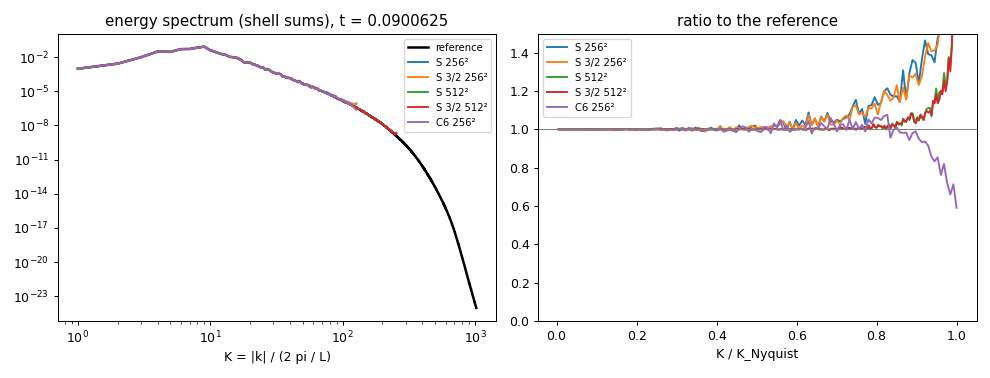
\includegraphics[width=0.95\textwidth]{padding.png}
\caption{Baseline spectra at $t=0.09$ for pseudospectral differentiation with and without $3/2$ padding on $256^2$ and $512^2$, together with C6 at $256^2$ and the $2048^2$ reference. The right panel shows the spectral ratio, clipped at 1.5. The padded and unpadded pseudospectral curves are almost indistinguishable.}
\label{fig:padding}
\end{figure}
Aliasing is an immediate candidate for explaining the pseudospectral accumulation near the cutoff. Without numerical attenuation at high wavenumber, nonlinear products can alias unresolved contributions back into the retained modes~\cite{kravchenko1997,moin1998}. The S$_{3/2}$ calculations provide a direct control for this mechanism. They remove quadratic aliasing of the nonlinear term from all retained non-Nyquist modes without reducing the available spectral interval.
The result is shown in \cref{tab:map,fig:padding}. In all ten cases, S${3/2}$ and S differ in $K{10}$ by no more than eight shells. Their high-wavenumber excess is also essentially unchanged: the largest values of $E/E_{\mathrm{ref}}$ remain between $1.6$ and $2.5$ with or without padding. Only one nominal leader changes, for $k_0=5$ on $256^2$, where S$_{3/2}$ reaches 109 shells compared with 105 for C6. No regime boundary moves.
For the skew-symmetric nonlinear form used here, quadratic aliasing is therefore not responsible for the pseudospectral pile-up or for the loss of bandwidth relative to C6 in the marginally resolved range. The skew-symmetric formulation is itself known to reduce aliasing errors~\cite{zang1991,blaisdell1996}, and the result should not be extended to the purely advective form without a separate test. What is established by the present control is narrower: the compact--spectral crossover remains when the retained non-Nyquist modes are dealiased by $3/2$ padding.
The remaining pile-up is consistent with an effect of spectral truncation. If enstrophy reaches the numerical cutoff faster than viscosity can remove it, energy can accumulate in the last retained modes, as occurs in Galerkin-truncated systems~\cite{cichowlas2005,frisch2008,ray2011}. Similar interpretations have been reported for alias-free three-dimensional calculations~\cite{ishihara2018}, and Bardos and Tadmor~\cite{bardos2015} showed that the 2/3 method can develop the same high-mode pathology as the aliased method once smoothness is lost. The structured search performed for this study found no previous control identical to the present padded/unpadded comparison on one marginally resolved flow. Nevertheless, these calculations only rule out quadratic nonlinear aliasing as the explanation; they do not establish the detailed mechanism of the remaining accumulation. A selective cutoff filter would provide one possible test of the truncation interpretation.
\subsection{Cost at equal resolved bandwidth}
\begin{table}[t]
\centering\small
\begin{tabular}{lcccccc}
\toprule
ms per GPU step & E6 (sparse) & E6, C6, S (Fourier) & S${2/3}$ & S${3/2}$ & C6, banded sparse \
\midrule
$256^2$ & 3.6 & 4.8 & 5.0 & 7.7 & 66 \
$512^2$ & 12.8 & 17.7 & 18.4 & 31.5 & 269 \
$1024^2$ & 51.8 & 78.5 & 82.0 & -- & -- \
\bottomrule
\end{tabular}
\caption{GPU time per step for decaying turbulence using the skew-symmetric nonlinear form and RK4. E6 is fastest as a sparse seven-point stencil. E6, C6 and S have the same cost when all are applied through Fourier symbols. The exact banded-circulant C6 implementation, with 78 and 45 entries per row, is approximately 15 times more expensive than the Fourier form. The $3/2$ treatment costs $1.85$ times the unpadded spectral step because five transforms are performed on grids of size $(3n/2)^2$ for each nonlinear evaluation.}
\label{tab:time}
\end{table}
The raw step times are given in \cref{tab:time}. When implemented through Fourier symbols, E6, C6 and S require essentially the same work per step. The sparse seven-point E6 implementation is about $1/1.4$ of this cost. The methods also differ in the maximum stable time step and in the spectral range obtained at a given $n$, so their ranking changes when cost is measured at equal effective bandwidth.
For $k_{\max}l_\eta\lesssim1$, E6 remains the least expensive of the tested under-resolved calculations. The corresponding equal-bandwidth estimates for C6 are $1.9$--$3.1$ times the E6 cost; those for S are $3.4$--$4.9$. Between approximately $k_{\max}l_\eta=1$ and $2.5$, C6 gives the lowest cost, at $0.44$--$0.74$ of E6, while S ranges from $0.64$ to $1.40$. In the best-resolved cases, $k_{\max}l_\eta\gtrsim2.5$, pseudospectral differentiation becomes the least expensive at equal bandwidth, with ratios of $0.54$--$0.76$. C6 remains competitive, at $0.69$--$0.81$.
Neither dealiased spectral variant is the cheapest by this metric. The 2/3 calculation costs between $1.3$ and $11$ times the equivalent-bandwidth E6 estimate. Padding retains the full pseudospectral range but increases each step by a factor of $1.85$. Consequently S${3/2}$ costs $1.00$--$1.31$ times E6 for $k{\max}l_\eta\ge2$ and approximately $2$--$9$ times E6 below this range. Even so, S${3/2}$ remains cheaper than S${2/3}$ at equal bandwidth in all cases, consistent with the results of Sinhababu and Ayyalasomayajula~\cite{sinhababu2021}. The quoted padded and unpadded timings, $31.5$ and $17.0,$ms on $512^2$, were obtained from the same build.
Where the higher-resolution schemes provide a cost advantage, the gains are generally of order tens of percent rather than orders of magnitude. Their additional resolved range is partly offset by a smaller allowable time step: approximately $20,%$ smaller for C6 and $50,%$ smaller for S relative to E6. These ratios apply to the skew-symmetric nonlinear form. Other formulations can alter the stability restriction; Raeth and Hallatschek~\cite{raeth2024}, for example, obtained a considerably tighter limit for spectral-like differentiation with an Arakawa Jacobian. All timings used here come from the same build, including a rerun of the baseline.
\subsection{Forced turbulence}
\label{sec:forced}
The forced cases are evaluated through time-averaged statistics because independently forced realizations decorrelate. Over the averaging intervals used here, the realized enstrophy input from the 28 forced modes varies by approximately $\pm8,%$. Differences of the same order cannot be separated reliably from this sampling variability.
For the hyperviscous case, all four methods give practically the same direct-cascade behavior. The measured spectral slopes range from $-3.44$ to $-3.48$, and the enstrophy-flux plateau ends at $K=66$ for every method, where hyperviscous dissipation becomes important. The plateau levels are 41.9, 43.0, 46.2 and 50.1 for E6, C6, S and S$_{2/3}$, respectively. Their variation is comparable to that of the total enstrophy removed in each realization and is therefore associated with the realized forcing input rather than with a measurable change of cascade dynamics. With dissipation confined close to the cutoff, no clear scheme dependence is observed in the inertial range.
The ordinary-viscosity case gives the same general conclusion. For $\Rey=10^5$ on $256^2$, the reference gives $k_{\max}l_\eta=1.33$ from the time-mean enstrophy dissipation and $\chi=2.8\times10^{-7}$. This lies in the range where C6 leads the decaying calculations. Each forced spectrum is normalized by its own enstrophy flux according to $E\propto\Pi_Z^{2/3}$ in order to remove the variation in realized input. The nominal $10,%$ bandwidths relative to the $768^2$ reference are $K=100$ for E6, 89 for S, 84 for C6 and 42 for S${2/3}$. Thus E6 has the largest nominal $K{10}$, unlike the decaying cases at similar $k_{\max}l_\eta$, but the remaining differences away from the cutoff are as large as $8,%$ and fall within the sampling uncertainty.
The principal differences are again concentrated near the end of the spectrum. At $K=120$, E6 has fallen to $0.64$ of the reference. The pseudospectral spectrum instead reaches $1.53$ and rises to about twice the reference at the Nyquist shell. C6 remains between these limits, with a ratio of $1.00$ at $K=120$ and an overshoot no larger than $17,%$ immediately below it, while S$_{2/3}$ terminates earlier. The close agreement of the inertial-range statistics is consistent with the forced-turbulence comparison reported by Rodhiya et al.~\cite{rodhiya2026}.
% =============================================================================
\section{Discussion}
% =============================================================================
The decaying calculations show that the cell Reynolds number is not sufficient to determine the relative behavior of the differentiation methods. Cases with the same $\Rey_c$ occupy different regimes because the small scales are set by the spectrum that develops in the flow, not by viscosity and grid spacing alone. The classical quantity $k_{\max}l_\eta$ contains this information through the realized enstrophy dissipation and arranges the leading method monotonically for the ten cases considered. The changes occur close to the values conventionally used to distinguish under-resolved, resolved and well-resolved two-dimensional calculations~\cite{lunasin2007}.
This result gives the familiar resolution criterion a second interpretation. In addition to indicating whether a calculation is sufficiently resolved, it also organizes which of the three differentiation approaches gives the largest reference-based bandwidth for its cost. This interpretation remains a posteriori in the present study because $l_\eta$ is obtained from the high-resolution reference. Scheme selection before a calculation would require a usable estimate of the enstrophy dissipation, and an under-resolved solution may itself give a poor value. This point has not been tested.
The result also clarifies the apparent difference from San and Staples~\cite{san2012}. Their sixth-order schemes agreed with the spectral method when the calculations were sufficiently resolved. Browning and Kreiss~\cite{browning1989} found a similar convergence of methods when the physical spectrum was concentrated well below the grid cutoff. The present bandwidth criterion examines agreement farther into the high-wavenumber range. In the best-resolved cases, pseudospectral differentiation consequently retains as much as $1.7$ times the E6 bandwidth. The cost comparison is also different: each method is timed directly in its fastest available implementation, and the estimate at equal bandwidth includes both the measured step time and the scheme-dependent stability limit. C6 and S require about $1.4$ times the sparse E6 step time, while $3/2$ padding requires $1.85$ times the unpadded spectral step.
The padded calculations address the origin of the pseudospectral cutoff accumulation separately. San and Staples observed high-wavenumber accumulation in non-conservative finite differences and associated it with aliasing. In the present calculations, the skew-symmetric form conserves enstrophy for every scheme. The finite-difference spectra fall below the reference near the cutoff, while the pseudospectral excess remains after $3/2$ padding. Quadratic aliasing of the nonlinear term is therefore not the cause of this pile-up for the formulation examined here. The remaining behavior is compatible with earlier descriptions based on spectral truncation~\cite{ishihara2018,bardos2015,frisch2008} and with dispersion-induced accumulation reported by Yalla et al.~\cite{yalla2021}, but the present tests do not establish which of these mechanisms is responsible.
The resulting scheme ordering has a simple numerical interpretation. When the grid does not resolve the enstrophy-dissipation scale, E6 is the least inaccurate method according to the present spectral-bandwidth measure. Its modified wavenumber substantially underestimates the exact derivative near the cutoff and supplies numerical attenuation. This behavior is useful only in the comparative sense: it does not recover absent scales and is not a replacement for increasing resolution. Vreman et al.~\cite{vreman1996} observed a related advantage of lower-order discretization under coarse filtering.
Once the dissipative scale is represented but is still close to the cutoff, C6 gives the best compromise. It extends the useful modified-wavenumber range substantially beyond E6 without retaining the exact high-wavenumber derivative of the pseudospectral method. This is the range $1\lesssim k_{\max}l_\eta\lesssim2$ in the present calculations, and corresponds closely to the marginal-resolution regime for which compact schemes were developed and applied by Laizet and Lamballais~\cite{laizet2009}. When the grid is well resolved, the exact spectral derivative becomes advantageous and the pseudospectral method gives the largest bandwidth at the lowest estimated cost.
Full dealiasing does not improve this cost balance for the cases tested. The 2/3 rule obtains exact conservation at the price of removing one third of the spectral interval. Padding retains the interval but raises the step cost by $85,%$, without materially changing the bandwidth in these runs. Other spectral treatments may give a different balance. Phase-shift dealiasing~\cite{lambert2026}, high-order Fourier filtering~\cite{hou2007} and selective filtering~\cite{yamamoto2026} were not examined here.
The organization by $k_{\max}l_\eta$ should not be interpreted as a general law for turbulent-flow statistics. It is obtained for transient decaying turbulence before the solutions decorrelate. The forced viscous case provides a direct limitation: at $k_{\max}l_\eta=1.33$, where C6 leads the decaying cases, E6 has the largest nominal $K_{10}$, but the differences are no larger than the sampling scatter and the inertial-range statistics do not distinguish the methods. The accuracy measure itself is also specific. Spectral bandwidth emphasizes agreement in $E(k)$; quantities such as structure functions, vortex statistics or higher-order moments may rank the schemes differently.
The use of Fourier symbols also provides a useful experimental control. On a periodic grid, finite-difference operators can be applied through the same spectral machinery as an exact derivative. The scheme then enters as a table of symbols, while the Poisson operator, diagnostics and transport terms remain consistent with that table. In particular, this avoids comparing a transport discretization with a Poisson operator representing a different numerical Laplacian. The approach is related to the mixed physical/spectral treatment of Laizet and Lamballais~\cite{laizet2009}. It also reduces the cost of the compact method considerably in the present periodic problem: the Fourier implementation is about 15 times faster than the exact banded circulant. This advantage is specific to periodic grids. For non-periodic or distributed problems, compact schemes require tridiagonal solutions, whose efficient implementation on CPUs and GPUs is a separate problem~\cite{akkurt2025}.
\paragraph{Limitations.}
The present study is restricted to two-dimensional periodic turbulence. Only one temporal scheme, classical RK4, and one nonlinear formulation, the skew-symmetric form, are considered. All performance measurements use double precision on one GPU, where FFT operations account for a large part of the computational cost.
The decaying matrix contains four variations about one baseline and gives ten values of $k_{\max}l_\eta$ after considering both grid sizes. It is sufficient to reveal the ordering reported here but not to determine sharp transition values. The two forced cases are additionally limited by sampling variability in the random forcing. Wall-bounded flows are outside the scope of this work; in such problems compact schemes require boundary closures and fully spectral methods no longer retain the simplicity of the periodic formulation. Selective filtering close to the cutoff, which Yamamoto and Tsuji~\cite{yamamoto2026} found effective in channel-flow calculations, was also not tested.
% =============================================================================
\section{Conclusions}
% =============================================================================
Explicit sixth-order, compact sixth-order and pseudospectral differentiation were compared for two-dimensional periodic turbulence using a common numerical framework. No method is preferable over the complete range of resolution studied. For transient decaying turbulence, the cell Reynolds number does not organize the ranking: calculations having the same $\Rey_c$ can give different leading schemes. A monotonic organization is instead obtained with the realized dissipation-scale resolution $k_{\max}l_\eta$, evaluated a posteriori from the high-resolution reference.
For $k_{\max}l_\eta\lesssim1$, the grid is under-resolved by the adopted criterion. E6 then gives the smallest spectral-bandwidth error and the lowest estimated cost among the methods tested, but it remains an under-resolved calculation and does not reproduce the missing scales. C6 is the leading method over the approximately resolved but not well-resolved range, $1\lesssim k_{\max}l_\eta\lesssim2$. Pseudospectral differentiation becomes preferable once the dissipative scale is well separated from the cutoff, at approximately $k_{\max}l_\eta\gtrsim2$--$2.5$. The changes occur near the usual thresholds for resolved and well-resolved two-dimensional calculations. A different wavenumber convention would rescale all values of $k_{\max}l_\eta$ together and therefore leave the ordering unchanged, although the numerical correspondence with those published thresholds would change.
The pseudospectral pile-up observed near the cutoff is not removed by $3/2$ padding. The padded and unpadded calculations give nearly the same bandwidth and high-wavenumber excess, while padding increases the step cost by a factor of $1.85$. For the skew-symmetric nonlinear form used here, the compact--spectral crossover is therefore not an artifact of quadratic aliasing of the nonlinear term. The remaining accumulation is compatible with truncation effects described in previous work, but its detailed mechanism was not established.
The regime map applies to the transient decaying cases considered and not to all turbulent statistics. In the forced calculation at $k_{\max}l_\eta=1.33$, the methods are indistinguishable in the inertial range within the forcing scatter and differ mainly near the cutoff. Further work is required to determine whether $l_\eta$ can be estimated reliably enough a priori to use the map for scheme selection, to place the transition values with additional cases, to examine other nonlinear formulations and to determine whether the same ordering occurs in three-dimensional turbulence.
\paragraph{Code and data availability.}
The cnavier repository (\url{https://github.com/leo-aa88/cnavier}) contains the solver, the analysis scripts (\code{tools/compare_schemes.py}, \code{tools/cascade.py} and \code{tools/modified_wavenumber.py}) and the command lines used for the simulations. A more detailed description of the implementation and verification tests is provided in \code{docs/cnavier_methodology.pdf}.
% =============================================================================
\begin{thebibliography}{99}
% =============================================================================
\bibitem{lele1992}
S.~K. Lele, Compact finite difference schemes with spectral-like resolution, \emph{J. Comput. Phys.} 103 (1992) 16--42.
\bibitem{laizet2009}
S.~Laizet, E.~Lamballais, High-order compact schemes for incompressible flows: a simple and efficient method with quasi-spectral accuracy, \emph{J. Comput. Phys.} 228 (2009) 5989--6015, doi:10.1016/j.jcp.2009.05.010.
\bibitem{laizet2011}
S.~Laizet, N.~Li, Incompact3d: a powerful tool to tackle turbulence problems with up to $O(10^5)$ computational cores, \emph{Int. J. Numer. Methods Fluids} 67 (2011) 1735--1757, doi:10.1002/fld.2480.
\bibitem{laizet2010}
S.~Laizet, E.~Lamballais, J.~C. Vassilicos, A numerical strategy to combine high-order schemes, complex geometry and parallel computing for high resolution DNS of fractal generated turbulence, \emph{Comput. Fluids} 39 (2010) 471--484.
\bibitem{bartholomew2020}
P.~Bartholomew, G.~Deskos, R.~A.~S. Frantz, F.~N. Schuch, E.~Lamballais, S.~Laizet, Xcompact3d: an open-source framework for solving turbulence problems on a Cartesian mesh, \emph{SoftwareX} 12 (2020) 100550.
\bibitem{ghosal1996}
S.~Ghosal, An analysis of numerical errors in large-eddy simulations of turbulence, \emph{J. Comput. Phys.} 125 (1996) 187--206, doi:10.1006/jcph.1996.0088.
\bibitem{kravchenko1997}
A.~G. Kravchenko, P.~Moin, On the effect of numerical errors in large eddy simulations of turbulent flows, \emph{J. Comput. Phys.} 131 (1997) 310--322, doi:10.1006/jcph.1996.5597.
\bibitem{moin1998}
P.~Moin, K.~Mahesh, Direct numerical simulation: a tool in turbulence research, \emph{Annu. Rev. Fluid Mech.} 30 (1998) 539--578.
\bibitem{san2012}
O.~San, A.~E. Staples, High-order methods for decaying two-dimensional homogeneous isotropic turbulence, \emph{Comput. Fluids} 63 (2012) 105--127, doi:10.1016/j.compfluid.2012.04.006.
\bibitem{rodhiya2026}
A.~Rodhiya, S.~Bhattacharya, M.~K. Verma, Relative accuracy of turbulence simulations using pseudo-spectral and finite difference solvers, \emph{S=adhan=a} 51 (2026) 38, doi:10.1007/s12046-025-03035-y.
\bibitem{orszag1971}
S.~A. Orszag, On the elimination of aliasing in finite-difference schemes by filtering high-wavenumber components, \emph{J. Atmos. Sci.} 28 (1971) 1074, doi:10.1175/1520-0469(1971)028<1074:OTEOAI>2.0.CO;2.
\bibitem{canuto2006}
C.~Canuto, M.~Y. Hussaini, A.~Quarteroni, T.~A. Zang, \emph{Spectral Methods: Fundamentals in Single Domains}, Springer, Berlin, 2006, doi:10.1007/978-3-540-30726-6.
\bibitem{fedioun2001}
I.~Fedioun, N.~Lardjane, I.~G"okalp, Revisiting numerical errors in direct and large eddy simulations of turbulence: physical and spectral spaces analysis, \emph{J. Comput. Phys.} 174 (2001) 816--851, doi:10.1006/jcph.2001.6939.
\bibitem{park2004}
N.~Park, J.~Y. Yoo, H.~Choi, Discretization errors in large eddy simulation: on the suitability of centered and upwind-biased compact difference schemes, \emph{J. Comput. Phys.} 198 (2004) 580--616, doi:10.1016/j.jcp.2004.01.017.
\bibitem{yalla2021}
G.~R. Yalla, T.~A. Oliver, R.~D. Moser, Numerical dispersion effects on the energy cascade in large-eddy simulation, \emph{Phys. Rev. Fluids} 6 (2021) L092601, doi:10.1103/PhysRevFluids.6.L092601.
\bibitem{frisch2008}
U.~Frisch, S.~Kurien, R.~Pandit, W.~Pauls, S.~S. Ray, A.~Wirth, J.-Z. Zhu, Hyperviscosity, Galerkin truncation, and bottlenecks in turbulence, \emph{Phys. Rev. Lett.} 101 (2008) 144501, doi:10.1103/PhysRevLett.101.144501.
\bibitem{yamamoto2026}
Y.~Yamamoto, Y.~Tsuji, A cost-effective pseudo-spectral scheme for high-Reynolds-number channel-flow DNS: accuracy, effective resolution, and computational cost under memory constraints, \emph{Comput. Fluids} 321 (2026) 107304, doi:10.1016/j.compfluid.2026.107304.
\bibitem{akkurt2025}
S.~Akkurt, S.~Lemaire, P.~Bartholomew, S.~Laizet, A distributed-memory tridiagonal solver based on a specialised data structure optimised for CPU and GPU architectures, \emph{Comput. Phys. Commun.} 315 (2025) 109747, doi:10.1016/j.cpc.2025.109747.
\bibitem{fox1973}
D.~G. Fox, S.~A. Orszag, Pseudospectral approximation to two-dimensional turbulence, \emph{J. Comput. Phys.} 11 (1973) 612--619, doi:10.1016/0021-9991(73)90141-1.
\bibitem{herring1974}
J.~R. Herring, S.~A. Orszag, R.~H. Kraichnan, D.~G. Fox, Decay of two-dimensional homogeneous turbulence, \emph{J. Fluid Mech.} 66 (1974) 417--444, doi:10.1017/S0022112074000280.
\bibitem{browning1989}
G.~L. Browning, H.-O. Kreiss, Comparison of numerical methods for the calculation of two-dimensional turbulence, \emph{Math. Comp.} 52 (1989) 369--388, doi:10.1090/S0025-5718-1989-0955748-0.
\bibitem{vreman1996}
B.~Vreman, B.~Geurts, H.~Kuerten, Comparison of numerical schemes in large-eddy simulation of the temporal mixing layer, \emph{Int. J. Numer. Methods Fluids} 22 (1996) 297--311, doi:10.1002/(SICI)1097-0363(19960229)22:4<297::AID-FLD361>3.0.CO;2-X.
\bibitem{yeung2018}
P.~K. Yeung, K.~R. Sreenivasan, S.~B. Pope, Effects of finite spatial and temporal resolution in direct numerical simulations of incompressible isotropic turbulence, \emph{Phys. Rev. Fluids} 3 (2018) 064603, doi:10.1103/PhysRevFluids.3.064603.
\bibitem{lunasin2007}
E.~Lunasin, S.~Kurien, M.~Taylor, E.~S. Titi, A study of the Navier--Stokes-$\alpha$ model for two-dimensional turbulence, \emph{J. Turbul.} 8 (2007) N30, doi:10.1080/14685240701439403.
\bibitem{baty2026}
H.~Baty, Triggering physical plasmoids in forming current sheets: conditions and diagnostics, arXiv:2604.02065 (2026), following J.~M. Garc'ia Morillo, A.~Alexakis, \emph{J. Fluid Mech.} 1007 (2025) R3, doi:10.1017/jfm.2025.109.
\bibitem{kritsuk2011}
A.~G. Kritsuk, \AA.~Nordlund, D.~Collins, P.~Padoan, M.~L. Norman, T.~Abel, R.~Banerjee, C.~Federrath, M.~Flock, D.~Lee, P.~S. Li, W.-C. M"uller, R.~Teyssier, S.~D. Ustyugov, C.~Vogel, H.~Xu, Comparing numerical methods for isothermal magnetized supersonic turbulence, \emph{Astrophys. J.} 737 (2011) 13, doi:10.1088/0004-637X/737/1/13.
\bibitem{fontana2020}
M.~Fontana, O.~P. Bruno, P.~D. Mininni, P.~Dmitruk, Fourier continuation method for incompressible fluids with boundaries, \emph{Comput. Phys. Commun.} 256 (2020) 107482, doi:10.1016/j.cpc.2020.107482.
\bibitem{cichowlas2005}
C.~Cichowlas, P.~Bona"iti, F.~Debbasch, M.~Brachet, Effective dissipation and turbulence in spectrally truncated Euler flows, \emph{Phys. Rev. Lett.} 95 (2005) 264502, doi:10.1103/PhysRevLett.95.264502.
\bibitem{ray2011}
S.~S. Ray, U.~Frisch, S.~Nazarenko, T.~Matsumoto, Resonance phenomenon for the Galerkin-truncated Burgers and Euler equations, \emph{Phys. Rev. E} 84 (2011) 016301, doi:10.1103/PhysRevE.84.016301.
\bibitem{bardos2015}
C.~Bardos, E.~Tadmor, Stability and spectral convergence of Fourier method for nonlinear problems: on the shortcomings of the 2/3 de-aliasing method, \emph{Numer. Math.} 129 (2015) 749--782, doi:10.1007/s00211-014-0652-y.
\bibitem{ishihara2018}
T.~Ishihara, N.~Kobayashi, K.~Enohata, M.~Umemura, K.~Shiraishi, Dust coagulation regulated by turbulent clustering in protoplanetary disks, \emph{Astrophys. J.} 854 (2018) 81, doi:10.3847/1538-4357/aaa976.
\bibitem{fornberg1987}
B.~Fornberg, The pseudospectral method: comparisons with finite differences for the elastic wave equation, \emph{Geophysics} 52 (1987) 483--501, doi:10.1190/1.1442319.
\bibitem{kawai2026}
Y.~Kawai, X.~Ren, S.~Nishizawa, T.~Katagiri, H.~Tomita, Comparison of computational advantages of high-order discontinuous Galerkin and conventional finite-volume dynamical cores in atmospheric turbulent simulations, \emph{J. Meteorol. Soc. Japan} 104 (2026) 20, doi:10.1007/s44394-026-00023-6.
\bibitem{raeth2024}
M.~Raeth, K.~Hallatschek, Surprisingly tight Courant--Friedrichs--Lewy condition in explicit high-order Arakawa schemes, \emph{Phys. Fluids} 36 (2024) 105167, doi:10.1063/5.0223009.
\bibitem{sinhababu2021}
A.~Sinhababu, S.~Ayyalasomayajula, Accuracy and computational efficiency of dealiasing schemes for the DNS of under resolved flows with strong gradients, \emph{Math. Comput. Simul.} 182 (2021) 116--142, doi:10.1016/j.matcom.2020.10.020.
\bibitem{lambert2026}
C.~Lambert, J.~Reneuve, P.~Augier, Aliasing and phase shifting in pseudo-spectral simulations of the incompressible Navier--Stokes equations, arXiv:2603.08892 (2026).
\bibitem{hou2007}
T.~Y. Hou, R.~Li, Computing nearly singular solutions using pseudo-spectral methods, \emph{J. Comput. Phys.} 226 (2007) 379--397, doi:10.1016/j.jcp.2007.04.014.
\bibitem{zang1991}
T.~A. Zang, On the rotation and skew-symmetric forms for incompressible flow simulations, \emph{Appl. Numer. Math.} 7 (1991) 27--40, doi:10.1016/0168-9274(91)90102-6.
\bibitem{blaisdell1996}
G.~A. Blaisdell, E.~T. Spyropoulos, J.~H. Qin, The effect of the formulation of nonlinear terms on aliasing errors in spectral methods, \emph{Appl. Numer. Math.} 21 (1996) 207--219, doi:10.1016/0168-9274(96)00005-0.
\end{thebibliography}
\end{document}
